\documentclass[11pt]{article}

\usepackage[letterpaper,margin=0.72in,headheight=15pt]{geometry}
\usepackage{amssymb}
\usepackage{array}
\usepackage{booktabs}
\usepackage{fancyhdr}
\usepackage{graphicx}
\usepackage{listings}
\usepackage{microtype}
\usepackage{tabularx}
\usepackage{tikz}
\usepackage{xcolor}
\usepackage[hidelinks]{hyperref}

\hypersetup
{
    pdftitle={ADK Lesson 004: PwmOutput and RgbLed},
    pdfauthor={Kevin Shanahan},
    pdfsubject={Safe PWM composition with a common-cathode RGB LED},
    pdflang={en-US}
}

\usetikzlibrary{arrows.meta,positioning}
\graphicspath{{docs/lessons/assets/}{../assets/}}

\definecolor{ink}{HTML}{20252A}
\definecolor{soft}{HTML}{F3F2EE}
\definecolor{mid}{HTML}{6F777B}
\definecolor{accent}{HTML}{3E5964}
\definecolor{codebg}{HTML}{F7F7F4}
\definecolor{wireR}{HTML}{8C3D3D}
\definecolor{wireG}{HTML}{3B7046}
\definecolor{wireB}{HTML}{3E5E83}

\pagestyle{fancy}
\fancyhf{}
\lhead{\textsc{ADK field lesson 004}}
\rhead{PWM and RGB composition}
\cfoot{\thepage}
\setlength{\parindent}{0pt}
\setlength{\parskip}{5pt}
\renewcommand{\arraystretch}{1.2}

\lstdefinestyle{adkcpp}
{
    language=C++,
    basicstyle=\ttfamily\small,
    backgroundcolor=\color{codebg},
    frame=single,
    rulecolor=\color{mid},
    columns=fullflexible,
    keepspaces=true,
    showstringspaces=false,
    keywordstyle=\bfseries\color{accent},
    commentstyle=\itshape\color{mid},
    breaklines=true,
    tabsize=4
}

\newcommand{\blankline}{\rule{0.96\linewidth}{0.35pt}}
\newcommand{\checkbox}{\(\square\)}

\newenvironment{checkpoint}[1]
{\begin{center}\begin{minipage}{0.94\linewidth}\textbf{Check --- #1}\par}
{\end{minipage}\end{center}}

\begin{document}

\begin{center}
    {\Huge\bfseries Compose three controlled currents}\\[3pt]
    {\Large Lesson 004: \texttt{PwmOutput} and \texttt{RgbLed}}\\[7pt]
    \textit{Calculate $\rightarrow$ wire $\rightarrow$ test $\rightarrow$ mix}
\end{center}

\begin{center}
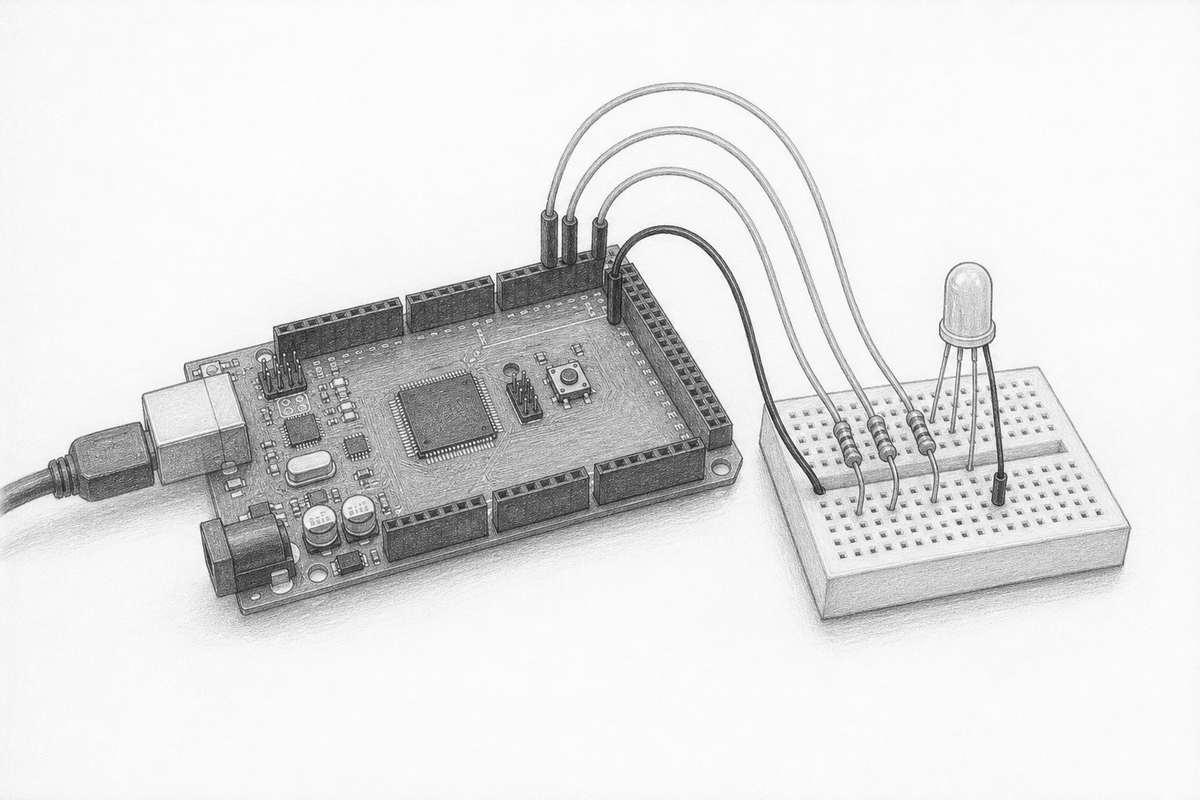
\includegraphics[width=\linewidth,height=0.30\textheight,keepaspectratio]
    {004-pwm-rgb-pencil.png}
\end{center}

\textbf{Orientation plate.}
Use the graphite view to recognize the parts and their approximate placement.
It is not a pin map. Breadboard connectivity and RGB LED leg order vary; the
exact circuit and your component's datasheet govern the build.

\begin{tabularx}{\linewidth}{@{}>{\bfseries}lX@{}}
Question & Can three owning PWM endpoints safely compose one deterministic
common-cathode RGB LED?\\
Time & 70--95 minutes\\
Prerequisites & Lessons 001--003; explicit status handling; resistor reading\\
You need & Mega 2560, USB cable, breadboard, common-cathode RGB LED, three
verified resistors, four jumpers, and a multimeter\\
Evidence & Current worksheet, exact host trace, color observations, and
high-impedance teardown\\
Safety class & E1: USB-powered Mega and current-limited LEDs only\\
Status & Host-verified and experimental; not yet hardware-accepted or stable\\
\end{tabularx}

\section*{Safety boundary}

Use only USB power and the low-energy circuit shown here. Remove every power
source before changing a wire. Never omit or share the three current-limiting
resistors. Confirm the LED is \emph{common cathode}; a common-anode part needs
different semantics and is outside this lesson.

\textbf{Stop} for heat, odor, smoke, unexpected USB disconnects, an unknown
resistor value, or an unidentified LED common lead. Disconnect USB upstream.
Do not troubleshoot a powered breadboard by moving jumpers.

\begin{checkpoint}{before wiring}
\checkbox\ USB removed \quad \checkbox\ LED datasheet or verified pinout \quad
\checkbox\ three resistors measured \quad \checkbox\ rails traced
\end{checkpoint}

\section*{1. Read the exact common-cathode circuit}

The cathodes of the three LED dies meet at one common lead connected to Mega
\texttt{GND}. Each anode has its \emph{own} series resistor. Pins 6, 5, and 3
are PWM-capable on the Mega 2560.

\begin{center}
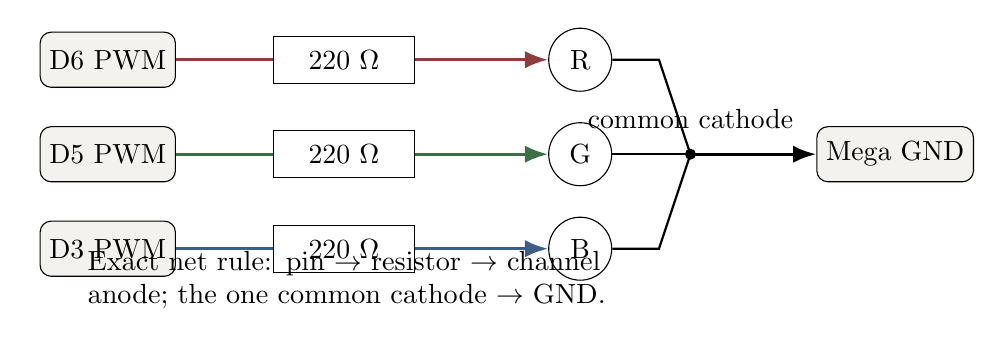
\begin{tikzpicture}[x=1cm,y=1cm,>=Latex,
    terminal/.style={draw,rounded corners,fill=soft,minimum width=17mm,
                     minimum height=7mm},
    resistor/.style={draw,minimum width=18mm,minimum height=6mm,fill=white}]
    \node[terminal] (p6) at (0,2.4) {D6 PWM};
    \node[terminal] (p5) at (0,1.2) {D5 PWM};
    \node[terminal] (p3) at (0,0.0) {D3 PWM};
    \node[resistor] (rr) at (3.0,2.4) {220 \(\Omega\)};
    \node[resistor] (rg) at (3.0,1.2) {220 \(\Omega\)};
    \node[resistor] (rb) at (3.0,0.0) {220 \(\Omega\)};
    \node[draw,circle,minimum size=8mm] (red) at (6.0,2.4) {R};
    \node[draw,circle,minimum size=8mm] (green) at (6.0,1.2) {G};
    \node[draw,circle,minimum size=8mm] (blue) at (6.0,0.0) {B};
    \coordinate (common) at (7.4,1.2);
    \node[terminal] (gnd) at (10.0,1.2) {Mega GND};
    \draw[very thick,wireR,->] (p6)--(rr)--(red);
    \draw[very thick,wireG,->] (p5)--(rg)--(green);
    \draw[very thick,wireB,->] (p3)--(rb)--(blue);
    \draw[thick] (red)--(7.0,2.4)--(common);
    \draw[thick] (green)--(common);
    \draw[thick] (blue)--(7.0,0.0)--(common);
    \fill (common) circle (2pt);
    \draw[very thick,->] (common)--(gnd);
    \node[above=2mm of common] {common cathode};
    \node[below=8mm of rg,text width=7.8cm,align=center] {
        Exact net rule: pin \(\rightarrow\) resistor \(\rightarrow\)
        channel anode; the one common cathode \(\rightarrow\) GND.};
\end{tikzpicture}
\end{center}

\begin{checkpoint}{continuity check while unpowered}
\checkbox\ no pin-to-pin short \quad \checkbox\ each channel has one resistor
\quad \checkbox\ common lead reaches GND only
\end{checkpoint}

\section*{2. Budget current before applying power}

Use the LED datasheet's forward voltage \(V_f\), not lens color or guesswork.
For a first estimate,
\[
I=\frac{V_{\rm pin}-V_f}{R}.
\]
With \(V_{\rm pin}=5.0\) V and \(R=220\,\Omega\), a red die at
\(V_f=2.0\) V estimates \(13.6\) mA; a green or blue die at \(3.0\) V
estimates \(9.1\) mA. All three at full duty estimate \(31.8\) mA total.
These are estimates, not guarantees: output voltage falls under load and
device limits are simultaneous constraints.

Repeat the calculation with the datasheet's \emph{minimum} \(V_f\), which
produces the largest current. Sum all three channels at duty 255. Do not apply
power unless each channel and the total remain below the documented operating
limits with margin.

\begin{center}
\begin{tabularx}{0.9\linewidth}{@{}lXXXX@{}}
\toprule
Channel & Measured \(R\) & Datasheet \(V_f\) & Estimated \(I\) & Accepted?\\
\midrule
red   & & & & \\
green & & & & \\
blue  & & & & \\
\midrule
Total at full duty & & & & \\
\bottomrule
\end{tabularx}
\end{center}

Do not design to the microcontroller's absolute maximum. Check the official
ATmega2560 and LED datasheets for per-pin, grouped-pin, total-device, and LED
limits. If any estimate lacks margin, increase resistance or stop.

\section*{3. Understand duty, not ``analog voltage''}

\texttt{PwmOutput::Duty} is an 8-bit value: 0 is always inactive, 255 is
always active, and intermediate values switch rapidly. Duty 128 is about
50\%, but it does not command a steady 2.5 V. The LED and eye integrate pulses.

\begin{center}
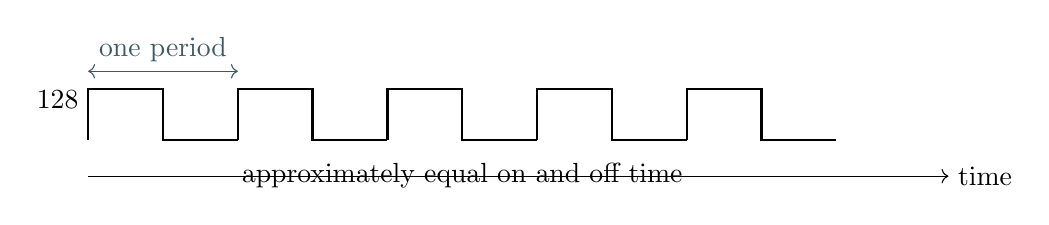
\begin{tikzpicture}[x=0.95cm,y=0.65cm]
    \draw[->] (0,0)--(11.5,0) node[right]{time};
    \node[left] at (0,1.5) {128};
    \foreach \x in {0,2,4,6,8}
    {
        \draw[thick] (\x,0.7)--(\x,1.7)--(\x+1,1.7)--(\x+1,0.7)--(\x+2,0.7);
    }
    \draw[<->,accent] (0,2.05)--node[above]{one period}(2,2.05);
    \node[below] at (5,0.45) {approximately equal on and off time};
\end{tikzpicture}
\end{center}

\textbf{Predict.} Order the apparent brightness for duties
0, 16, 64, 128, and 255:
\par\blankline

\section*{4. Read the exact endpoint API}

\texttt{PwmOutput} claims one PWM-capable Mega pin. Initialization writes the
initial duty. Shutdown writes zero, selects input mode, and releases the claim.
All operations are exception-free; destruction performs idempotent shutdown.

\begin{lstlisting}[style=adkcpp]
adk::Runtime   runtime;
adk::PwmOutput red (runtime.resources (), 6, 0);

adk::Status status = red.initialize ();
if (status == adk::Status::Ok)
{
    status = red.write (128);
}

red.shutdown ();
\end{lstlisting}

An invalid pin reports \texttt{InvalidPin}; a valid non-PWM pin reports
\texttt{Unsupported}; a claimed pin reports \texttt{ResourceBusy}; writing
before initialization reports \texttt{NotInitialized}.

\section*{5. Compose the semantic RGB component}

\texttt{RgbLed} owns three \texttt{PwmOutput} objects. Its channel descriptors
retain both pin identity and the documented resistor value. For a
common-cathode LED, color byte values map directly to duty.

\begin{lstlisting}[style=adkcpp]
adk::Runtime runtime;
adk::RgbLed  led (runtime.resources (),
                  {6, 220},
                  {5, 220},
                  {3, 220});

if (led.initialize () == adk::Status::Ok)
{
    led.set (adk::Rgb (255, 64, 0));
    led.off ();
}
\end{lstlisting}

Initialization is transactional: red, green, and blue claims must all succeed.
A later failure releases earlier claims. \texttt{set()} updates all three
channels; \texttt{off()} sets \texttt{Rgb(0,0,0)}. Shutdown proceeds through
the owned endpoints, leaving every channel at zero and high impedance.

\begin{center}
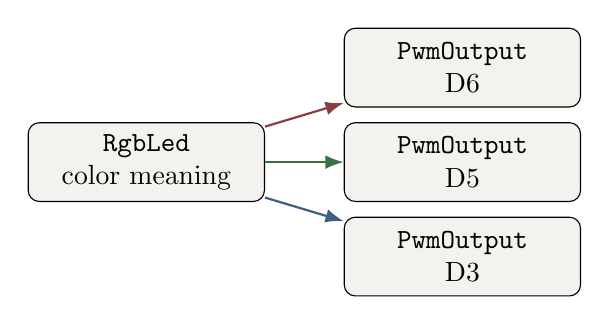
\begin{tikzpicture}[>=Latex,node distance=10mm,
    box/.style={draw,rounded corners,fill=soft,minimum width=30mm,
                minimum height=10mm,align=center}]
    \node[box] (rgb) {\texttt{RgbLed}\\color meaning};
    \node[box,right=of rgb,yshift=12mm] (r) {\texttt{PwmOutput}\\D6};
    \node[box,right=of rgb] (g) {\texttt{PwmOutput}\\D5};
    \node[box,right=of rgb,yshift=-12mm] (b) {\texttt{PwmOutput}\\D3};
    \draw[->,wireR,thick] (rgb)--(r);
    \draw[->,wireG,thick] (rgb)--(g);
    \draw[->,wireB,thick] (rgb)--(b);
\end{tikzpicture}
\end{center}

\section*{6. Prove behavior on the host}

The fake Arduino trace is the electrical contract's executable evidence.
Write tests for:

\begin{enumerate}
    \item every Mega PWM pin and representative valid non-PWM pins;
    \item duty endpoints 0 and 255 plus one intermediate value;
    \item write before initialization and repeated initialization;
    \item duplicate claims, release, and reuse;
    \item destruction: \texttt{analogWrite(pin, 0)} before
          \texttt{pinMode(pin, INPUT)};
    \item RGB initialization failure on the second and third channel;
    \item exact red--green--blue write order for several colors;
    \item repeated \texttt{off()} and \texttt{shutdown()};
    \item two identical runs producing identical traces.
\end{enumerate}

\textbf{Trace exercise.} Predict the complete operation trace for
\texttt{RgbLed::initialize()}, \texttt{set(Rgb(255,64,0))}, and destruction:

\blankline\\[5pt]\blankline\\[5pt]\blankline

\section*{7. Build and observe}

Run the repository's host checks and compile the canonical Mega example before
upload. Inspect every status; an ignored failure makes observations ambiguous.

\begin{lstlisting}[style=adkcpp]
make check
make arduino
arduino-cli board list
\end{lstlisting}

\begin{enumerate}
    \item Remove USB. Build and continuity-check the exact circuit.
    \item Connect USB only. Upload to the port you explicitly identified.
    \item Command red, green, blue, white, off, and one mixed color.
    \item Record observed color and whether any channel appears swapped.
    \item Run the shutdown phase. Confirm all channels are inactive.
    \item Remove USB before correcting any channel identity.
\end{enumerate}

\begin{center}
\begin{tabularx}{\linewidth}{@{}lXXX@{}}
\toprule
Command & Expected & Observed & Trace/status\\
\midrule
\texttt{Rgb(255,0,0)}   & red   & &\\
\texttt{Rgb(0,255,0)}   & green & &\\
\texttt{Rgb(0,0,255)}   & blue  & &\\
\texttt{Rgb(255,255,255)} & combined white & &\\
\texttt{Rgb(0,0,0)}     & off & &\\
\bottomrule
\end{tabularx}
\end{center}

\section*{8. Explain what the abstraction prevents}

\begin{enumerate}
    \item Why must each die have a separate resistor?
    \item Why does common cathode permit direct duty semantics?
    \item Why should \texttt{RgbLed} compose rather than inherit from
          \texttt{PwmOutput}?
    \item What must happen if the blue pin is already claimed?
    \item Why is a stored resistor value useful even though software cannot
          enforce the physical resistor?
    \item Which evidence proves teardown better than visual darkness?
\end{enumerate}

\section*{Exit ticket}

\checkbox\ circuit checked unpowered \quad
\checkbox\ current budget recorded \quad
\checkbox\ host tests pass \quad
\checkbox\ Mega build passes \quad
\checkbox\ status paths handled \quad
\checkbox\ teardown trace verified

\vfill
\small
\textbf{Companion material.}
Use the HTML lesson for exact source links, current API signatures, errata,
Mega pin-capability tables, and authoritative datasheet links. Use this PDF
for bench predictions, wiring checks, calculations, observations, and sign-off.
This lesson remains host-verified until its physical acceptance record is
published.

\href{https://docs.arduino.cc/hardware/mega-2560/}
{Arduino Mega 2560 documentation}\quad
\href{https://www.microchip.com/en-us/product/ATmega2560}
{Microchip ATmega2560 datasheet}

\end{document}
